\chapter{Supplementary material}\label{App1}

%\clearpage
%\begin{figure}[ht]
%	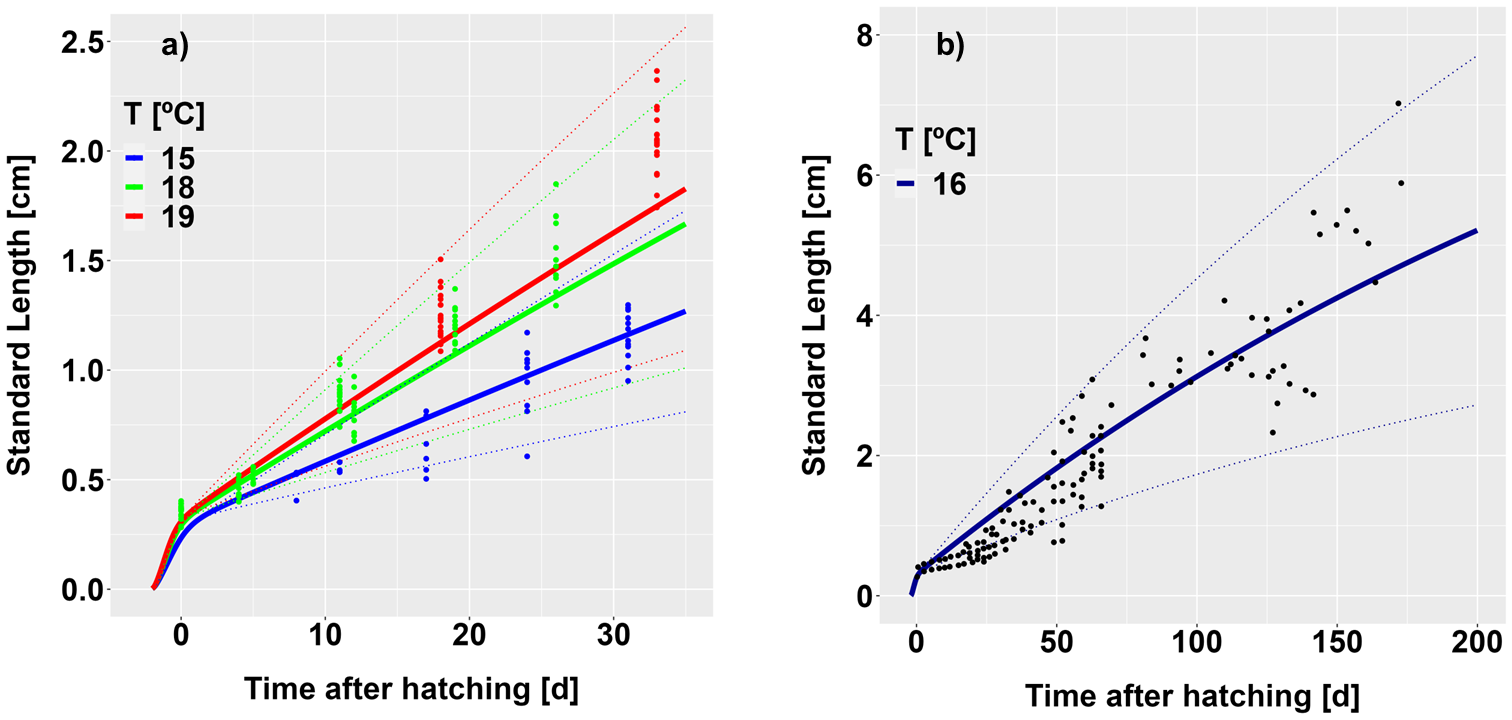
\includegraphics[width=1.0\textwidth]{figures/S1DEBvsData.png}
%	\centering
%	\caption{Comparison of Peruvian anchovy simulated larval growth and laboratory observations from \cite{RiouOfel2021} (a) and in situ observations from \cite{MoreClar2011} (b). Thick lines correspond to average size predictions considering ten $f$ values from 0.1 to 1 with 0.1 steps (food limitation factor, see section 2.1.6) at $19$\textdegree $C$ (red), $18$\textdegree $C$ (green) and $15$\textdegree $C$ (blue) in (a) and at $16$\textdegree C in (b). Dotted lines correspond to standard deviation of the simulated larval growth. Colored dots show the corresponding observations. The bioenergetic model parameters were taken from \cite{PethRoos2013}. Note that the scales are different in the two panels.}
%	\label{S1DEBvsData}
%\end{figure}

%\section{Standard $DEB_{std}$ Equations in Ichthyop-DEB model}\label{DEBstdEqn}
%
%Jorge Flores-Valiente et al.\\
%
%The following description is a simplification of the \gls{encrasicolus} \acrshort{deb} model developed by \cite{PethRoos2013} as we only focus on the embryo and larva stages. We implemented these equations in the Lagrangian tool routines of \gls{ich} \citep{LettVerl2008} to develop \gls{ich-deb}.\\
%
%\begin{figure}[ht]
%	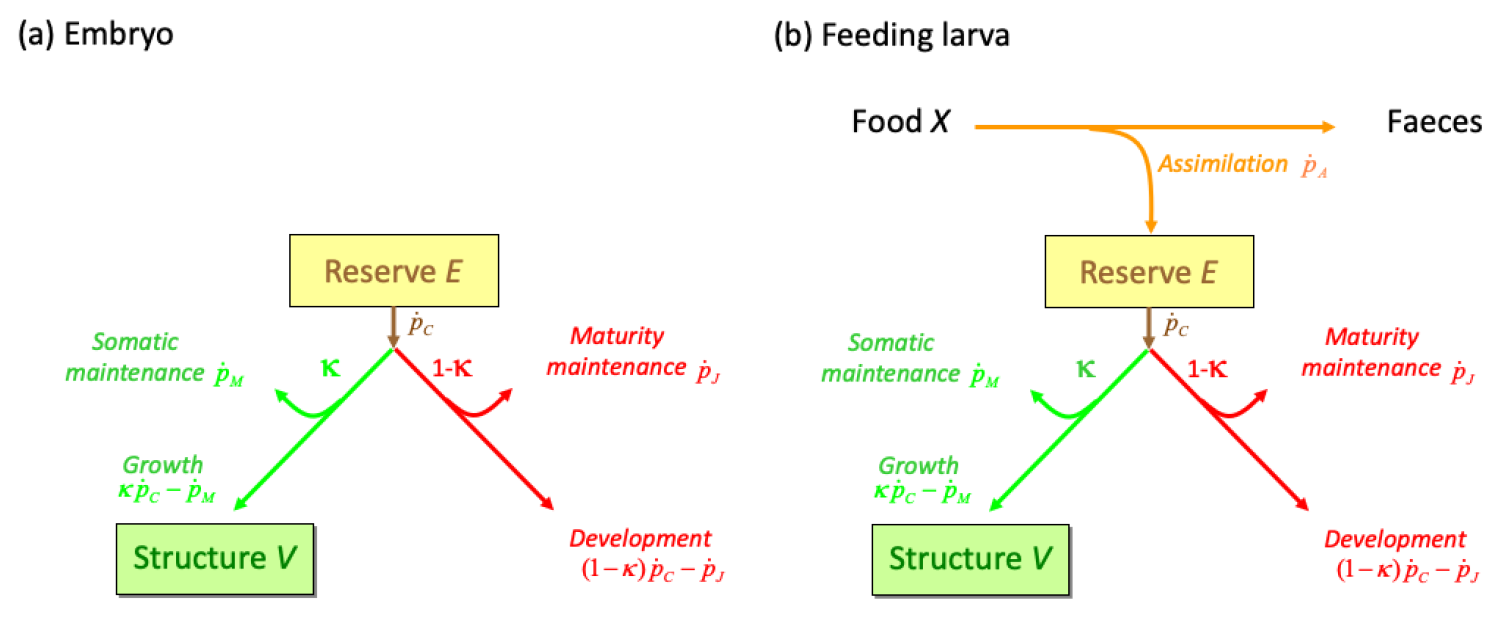
\includegraphics[width=1.0\textwidth]{figures/S1DEBflux.png}
%	\centering
%	\caption{Schemes of the energy fluxes of a \acrlong{deb} model (a) for the embryo stage (non-feeding stage) and (b) the feeding larval stage.}
%	\label{S1DEBflux}
%\end{figure}
%
%\subsection*{Forcing variables}
%\hfill \\
%
%$T$ Temperature (K) is the water temperature surrounding an individual (modeled by CROCO-PISCES)\\
%
%$X$ Food density averaged Mesozooplankton field ($\left[ \mu mol CL^{-1} \right]$) over the water column (modeled by CROCO-PISCES)\\
%
%\subsection*{Initial conditions of state variables (egg stage)}
%
%The age of the individual is set at zero on the day of spawning.\\
%
%\begin{tabular}{|c|c|c|c|}
%\hline 
%Symbol  & Value      & Units  & Definition      \\ 
%\hline 
%$E$     & $0.99$     & $J$    & Initial Reserve \\ 
%$V$     & $0.000001$ & $mm^3$ & Initial Structure\\
%\hline 
%\end{tabular} 
%
%\subsection*{Primary parameters}
%
%\begin{table}[H]
%\centering
%\begin{adjustbox}{width=1.2\textwidth}
%\begin{tabular}{l|l|l|l}
%\hline
%\multicolumn{4}{l}{Primary parameters (rates are at reference temperature $T_{1} = 293 K$  ($=20$\textdegree $C$)} \\
%\hline
%Symbol   & Value        & Unit & Definition                                \\
%\hline
%$L_{h}$  & 0.28         & $cm$ & Hatch length                              \\
%$L_{b}$  & 0.35         & $cm$ & Yolk-sac to feeding larva threshold       \\
%$T_{A}$  & 9800         & $K$  & Arrhenius temperature                     \\
%$T_{L}$  & 279/279      & $K$  & Lower temperature boundary                \\
%$T_{H}$  & 294/297      & $K$  & Upper temperature boundary                \\
%$T_{AL}$ & 20000/20000  & $K$  & Arrhenius temperature for lower boundary  \\
%$T_{AH}$ & 95000/570000 & $K$  & Arrhenius temperature for upper boundary   \\
%$K$      & 1.6          & $\mu mol CL^{-1}$ & Half-saturation constant       \\
%$\kappa_{\mathrm{x}}$   & 0.71 & - & Fraction of food energy fixed in reserve \\
%$\left\{\dot{p}_\mathrm{Xm} \right\}$
%	& 516
%	& $J.cm^{-2}.d^{-1}$
%	& Maximum surface-specific ingestion rate         \\
%$\left[E_{m} \right]$
%	& 2700 
%	& $J.cm^{-3}$
%	& Maximum reserve density                         \\
%$\left[E_{G} \right]$
%	& 4000
%	& $J.cm^{-3}$
%	& Volume-specific costs of structure              \\
%$\left[\dot{p}_{M} \right]$
%	& 76.22 
%	& $J.cm^{-3}.d^{-1}$
%	& Volume-specific somatic maintenance rate\\
%$\kappa$
%	& 0.7
%	& - 
%	& Fraction of mobilized reserve allocated to growth and somatic maintenance    \\
%\hline
%\end{tabular}
%\end{adjustbox}
%\end{table}
%
%\subsection*{Auxiliary and compounds parameters}
%
%\begin{table}[H]
%\centering
%\begin{adjustbox}{width=1.2\textwidth}
%\begin{tabular}{l|l|l|l}
%\hline
%\multicolumn{4}{l}{Auxiliary and Compounds parameters}   \\
%\hline
%Symbol & Value & Unit & Definition                   \\
%$\delta_{M}$
%	& 0.152
%	& -
%	& Shape coefficient                               \\
%$\left \{ \dot{p}_\mathrm{Am} \right \}$
%	& $\kappa_{\mathrm{x}} $ $\left \{ \dot{p}_\mathrm{Xm} \right \}=366$
%	& $J.cm^{-2}.d^{-1}$
%	& Maximum surface-area-specific assimilation rate\\
%\hline
%\end{tabular}
%\end{adjustbox}
%\end{table}
%
%\subsection*{Scaled functional response}
%\hfill \\
%
%$V_{b} = (\delta_{M}L_{b})^3$ \hfill Structural volume at first-feeding in $cm^3$.\\
%
%\textbf{if} $(V < V_{b})$ \\
%
%$f = 0$ \hfill No feeding.\\
%
%\textbf{else}\\
%
%$f= \frac{X}{X+K}$	    \hfill Feeding.\\
%
%\subsection*{Temperature correction}
%\hfill \\
%
%Each rate parameter is corrected for temperature according to the following equation \citep{Kooi2009}.\\
%
%$
%	C_{T} = exp\left ( \frac{T_{A}}{T_{1}} - \frac{T_{A}}{T} \right )
%	\left ( \frac
%				{1+exp\left ( \frac{T_{AL}}{T_{1}} - \frac{T_{AL}}{T_{L}} \right )
%				  +exp\left ( \frac{T_{AH}}{T_{H}} - \frac{T_{AH}}{T_{1}} \right )}
%				{1+exp\left ( \frac{T_{AL}}{T} - \frac{T_{AL}}{T_{L}} \right )
%				  +exp\left ( \frac{T_{AH}}{T_{H}} - \frac{T_{AH}}{T} \right )}
%	\right )
%$\\
%
%With $T_{1}$ the reference temperature (at which flux parameters were estimated), $T_{A}$ is the Arrhenius temperature and $T_{AH}$, $T_{AH}$, $T_{L}$, $T_{H}$ are constants used to define a curved shape of the temperature correction according to temperature.\\
%
%$\left \{ \dot{p}_\mathrm{Am} \right \}_{T} = C_{T} \left \{ \dot{p}_\mathrm{Am} \right \}_{T_{1}}$\\
%
%$\left [ \dot{p}_{M} \right ]_{T} = C_{T} \left [ \dot{p}_{M} \right ]_{T_{1}}$\\
%
%\subsection*{Fluxes ($Jd^{-1}$)}
%\hfill \\
%
%$\dot{p}_\mathrm{A} = f \left \{ \dot{p}_\mathrm{Am} \right \}_{T} V^{2/3}$ \hfill Assimilation.\\
%
%$\dot{p}_\mathrm{M} = \left [ \dot{p}_{M} \right ]_{T} V$ \hfill Volume-related somatic maintenance.\\
%
%
%	$\dot{p}_{C} = \frac
%					   {E\left ( \left [ E_{G} \right ] \frac{C_{T}\left \{ \dot{p}_\mathrm{Am} \right \}_{T}}{\left [ E_{m} \right ]} V^{-\frac{1}{3}}+\left [ \dot{p}_{M} \right ]_{T}\right )}
%					   {\kappa\left ( \frac{E}{V} \right ) + \left [ E_{G} \right ]}$ \hfill Mobilization of energy.\\
%
%$\dot{p}_{G} = \kappa \dot{p}_{C} - \dot{p}_\mathrm{M}$ \hfill Energy directed to structural growth.\\
%
%$\dot{p}_{J} = V \frac{\left ( 1 - \kappa \right )}{\kappa}\left [ \dot{p}_{M} \right ]_{T}$ \hfill Maturity maintenance (for $V < V_{p}$ (Structural volume at puberty), the condition is always TRUE because in \gls{ich-deb} the complexity level of the organism at puberty is never exceeded, as we only consider embryos and larvae).\\
%
%Starvation test\\
%
%\textbf{if} $\kappa \dot{p}_{C} < \dot{p}_\mathrm{M}$ or $\left ( 1- \kappa \right ) \dot{p}_{C} < \dot{p}_{J}$\\
%
%$starvation = 1$ \hfill Individual (or super-individual) removed from population.\\
%
%\textbf{else}\\
%
%$starvation = 0$ \hfill Individual continues in the simulation.\\
%
%\subsection*{Differential equations}
%\hfill \\
%
%$\frac{dE}{dt} = \dot{p}_\mathrm{A} - \dot{p}_{C}$ \hfill Reserve dynamics.\\
%
%$\frac{dV}{dt} = \frac{\dot{p}_{G}}{\left[ E_{G} \right]}$ \hfill Structure dynamics.\\
%
%\subsection*{Integration}
%\hfill \\
%
%$E\left ( t + \Delta t \right ) = E\left ( t \right ) + \frac{dE}{dt}\Delta t$ \\
%
%$V\left ( t + \Delta t \right ) = V\left ( t \right ) + \frac{dV}{dt}\Delta t$ \\
%
%With $\Delta t = 0.083 d \left (=2hours\right )$
%
%\subsection*{Observable variables}
%\hfill \\
%
%$L_{w} = \frac{V^{1/3}}{\delta_{M}}$ \hfill Physical length ($cm$).\\
%
%where $L_{w}$ is the standard length $SL$ ($cm$), $V$ the structural volume ($cm^3$) and $\delta_{M}$ a shape coefficient.\\
%
%We assume that the larva does not change in shape till it reaches our length criteria of $2cm(SL)$ and that there is a constant proportionality ($\delta_{M}$) between structural volume and length.\\

\clearpage
\section{Accelerated $DEB_{abj}$ Equations in Ichthyop-DEB model}\label{DEBabjEqn}

Jorge Flores-Valiente et al.\\

This section describes the complete life cycle \acrshort{deb} model for \gls{ringens}, with a focus on the egg and larval periods. We implemented these equations in the Lagrangian tool routines of \gls{ich} \citep{LettVerl2008} to develop \gls{ich-deb}.\\

Table \ref{param_compar} presents a comparative list of parameters used in both bioenergetic models (\textit{\gls{encrasicolus}} and \textit{\gls{ringens}}) at a reference temperature $T_{1} = 293 K$  ($=20$\textdegree $C$).\\

% Tabla
\begin{table}[H]
\centering
\begin{adjustbox}{width=1.2\textwidth}
\begin{tabular}{c|c|c|c|l}
\hline
\multicolumn{5}{c}{Primary parameters (rates are at reference temperature $T_{1} = 293 K$  ($=20$\textdegree $C$)}\\
\hline
Symbol      & \textit{E. encrasicolus} & \textit{E. ringens}   & Unit   & Definition\\
\hline
$L_{1}$     & 0.28    & -        & $cm$     & Hatch length\\
$L_{2}$     & 0.35    & -        & $cm$     & Length at first-feeding\\
$E_{H}^{b}$ & -       & 0.335    & $J$      & Maturity threshold at birth\\
$E_{H}^{j}$ & -       & 83.22    & $J$      & Maturity threshold at metamorphosis\\
$E_{H}^{p}$ & -       & 42160    & $J$      & Maturity threshold at puberty\\
$L_{b}$      & - & 0.1038        & $cm$ & Volumetric length at birth (estimated at $f$ = 1)\\
$L_{j}$      & - & 0.6093        & $cm$ & Volumetric length at metamorphosis (estimated at $f$ = 1) \\
$T_{A}$     & 9800     & 10000   & $K$      & Arrhenius temperature\\
$T_{L}$     & 279      & 279     & $K$      & Lower temperature boundary\\
$T_{H}$     & 294(297) & 294(297)& $K$      & Upper temperature boundary\\
$T_{AL}$    & 20000    & 20000   & $K$      & Arrhenius temperature for lower boundary\\
$T_{AH}$    & 95000(570000)      & 95000(570000) & $K$ & Arrhenius temperature for upper boundary\\
$\kappa_{\mathrm{x}} $
	& 0.71
	& 0.8
	& -
	& Fraction of food energy fixed in reserve\\
$\left \{ \dot{p}_\mathrm{Xm} \right \}$
	& 516
	& $\left \{ \dot{p}_\mathrm{Am} \right \}/\kappa \mathrm{x} = 106(622)$
	& $J.cm^{-2}.d^{-1}$
	& \makecell[l]{Maximum surface specific ingestion rate \\ (before and after metamorphosis for \textit{E. ringens})} \\
$\left \{ \dot{p}_\mathrm{Am} \right \}$
	& $ \kappa \mathrm{x} \left \{ \dot{p}_\mathrm{Xm} \right \}= 366$
	& 84.97(498)
	& $J.cm^{-2}.d^{-1}$
	& \makecell[l]{Surface-area-specific maximum assimilation rate \\ (before and after metamorphosis for \textit{E. ringens})} \\
$\left[ E_{m} \right]$ 
	& 2700
	& $\left \{ \dot{p}_\mathrm{Am} \right \}/\dot{v}=2060$
	& $J.cm^{-3}$ & Maximum reserve density\\
$\left[ E_{G} \right]$
	& 4000
	& 5283
	& $J.cm^{-3}$ & Volume-specific costs of structure\\
$\left [ \dot{p}_{M} \right ]$
	& 76.22
	& 79.95
	& $J.cm^{-3}.d^{-1}$
	& Specific Volume-linked somatic maintenance rate\\
$\kappa$
	& 0.7 
	& 0.5512 
	& - 
	& Fraction of mobilized reserve allocated to soma\\
$\dot{k}_{J}$ & - & 0.002 	        & $d^{-1}$     & Maturity maintenance rate coefficient\\
$\dot{v}$
	& - & 0.04124(0.2421)
	& $cm. d^{-1}$ 
	& \makecell[l]{Energy conductance \\ (before and after metamorphosis for \textit{E. ringens})}\\
$\delta_{M}$
	& 0.152
	& 0.1889
	& -
	& Shape coefficient for larvae\\
\end{tabular}
\end{adjustbox}
\end{table}


\subsection*{Forcing variables}
\hfill \\

$T$ Temperature (K) is the water temperature surrounding an individual (modeled by CROCO-PISCES)\\

$X$ Food density averaged Mesozooplankton field ($\left[ \mu mol CL^{-1} \right]$) over the water column (modeled by CROCO-PISCES)\\

\subsection*{State variables – Initial conditions}

The age of the individual is set at zero on the day of spawning.\\

\begin{tabular}{|c|c|c|c|}
\hline 
Symbol  & Value      & Units  & Definition      \\ 
\hline 
$E$     & $0.99$     & $J$    & Initial Reserve \\ 
$V$     & $0.000001$ & $mm^3$ & Initial Structure\\
$E_{H}$ & $0$ 		  & $J$    & Cumulated energy invested into development\\
$E_{R}$ & $0$         & $J$   & Reproduction buffer\\
\hline 
\end{tabular}

\subsection*{Scaled functional response}
\hfill \\

\textbf{if} $(E_{H} < E_{H}^b)$\\

$f = 0$				\hfill No feeding.\\

\textbf{else}\\

$f= \frac{X}{X+K}$	\hfill Feeding.\\

\subsection*{Temperature correction}
\hfill \\

Each rate parameter is corrected for temperature according to the following equation \citep{Kooi2009}.\\

$
	C_{T} = exp\left ( \frac{T_{A}}{T_{1}} - \frac{T_{A}}{T} \right )
	\left ( \frac
				{1+exp\left ( \frac{T_{AL}}{T_{1}} - \frac{T_{AL}}{T_{L}} \right )
				  +exp\left ( \frac{T_{AH}}{T_{H}} - \frac{T_{AH}}{T_{1}} \right )}
				{1+exp\left ( \frac{T_{AL}}{T} - \frac{T_{AL}}{T_{L}} \right )
				  +exp\left ( \frac{T_{AH}}{T_{H}} - \frac{T_{AH}}{T} \right )}
	\right )
$\\

With $T_{1}$ the reference temperature (at which flux parameters were estimated), $T_{A}$ is the Arrhenius temperature and $T_{AH}$, $T_{AH}$, $T_{L}$, $T_{H}$ are constants used to define a curved shape of the temperature correction according to temperature.\\

$\left \{ \dot{p}_\mathrm{Am} \right \}_{T} = C_{T} \left \{ \dot{p}_\mathrm{Am} \right \}_{T_{1}}$\\

$\left [ \dot{p}_{M} \right ]_{T} = C_{T} \left [ \dot{p}_{M} \right ]_{T_{1}}$\\


Temperature correction now affects two additional parameters.\\

$\dot{v}_{T} = C_{T} \dot{v}_{T_{1}}$\\

$\dot{K}_{jT} = C_{T} \dot{K}_{jT_{1}}$\\

\subsection*{Metabolic acceleration}
\hfill \\

Only two parameters are impacted by growth acceleration.\\

\textbf{if}	$E_{H} < E_{H}^b$\\

$S_{M} = 1$ \hfill No acceleration.\\

\textbf{else if} $E_{H}^b < E_{H} < E_{H}^j$\\

$S_{M} = \frac{L}{L_{b}}$ \hfill Acceleration.\\

\textbf{else}\\

$S_{M} = \frac{L_{j}}{L_{b}}$ \hfill Constant growth.\\

The $S_{M}$ parameter only accelerates growth from birth to metamorphosis.\\

$\left \{ \dot{p}_\mathrm{Am} \right \}_{S_{M}} = S_{M} \left \{ \dot{p}_\mathrm{Am} \right \}_{T}$\\

$\dot{v}_{S_{M}} = S_{M} \dot{K}_{jT}$\\

\subsection*{Fluxes ($Jd^{-1}$)}
\hfill \\

\textbf{if}	$E_{H} < E_{H}^b$\\

$\dot{p}_\mathrm{A} = 0$ \hfill No assimilation.\\

\textbf{else}\\

$\dot{p}_\mathrm{A} = f \left \{ \dot{p}_\mathrm{Am} \right \}_{S_{M}} V^{2/3}$ \hfill Assimilation.\\

\hfill \\

$\dot{p}_\mathrm{M} = \left [ \dot{p}_{M} \right ]_{T} V$ \hfill Volume-related somatic maintenance.\\

$\dot{p}_{C} = \frac{E}{V}*\frac{\left [ E_{G} \right ]\dot{v}_{S_{M}}V^{2/3}+\left [ \dot{p}_{M} \right ]_{T}}{\kappa\frac{E}{V}+\left [ E_{G} \right ]}$ \hfill Mobilization of energy.\\

$\dot{p}_{J} = \dot{K}_{jT} E_{H}$ \hfill Maturity maintenance.\\

\subsection*{Differential equations}
\hfill \\

$\frac{dE}{dt} = \dot{p}_\mathrm{A} - \dot{p}_{C}$ \hfill Reserve dynamics.\\

$\frac{dV}{dt} = \frac{\kappa \dot{p}_{C} - \dot{p}_\mathrm{M}}{\left[E_{G} \right]}$\\

\textbf{if} $E_{H} < E_{H}^p$\\

$\frac{dE_{H}}{dt} = (1 - \kappa) \dot{p}_{C} - \dot{p}_{J}$\\

$\frac{dE_{R}}{dt} = 0$\\

\textbf{else}\\

$\frac{dE_{H}}{dt} = 0$\\

$\frac{dE_{R}}{dt} = (1 - \kappa) \dot{p}_{C} - \dot{p}_{J}$\\

\subsection*{Integration}
\hfill \\

$E\left ( t + \Delta t \right ) = E\left ( t \right ) + \frac{dE}{dt}\Delta t$ \\

$V\left ( t + \Delta t \right ) = V\left ( t \right ) + \frac{dV}{dt}\Delta t$ \\

$E_{H}\left ( t + \Delta t \right ) = E_{H}\left ( t \right ) + \frac{dE_{H}}{dt}\Delta t$ \\

$E_{R}\left ( t + \Delta t \right ) = E_{R}\left ( t \right ) + \frac{dE_{R}}{dt}\Delta t$ \\

With $\Delta t = 0.083 d \left (=2hours\right )$

\subsection*{Observable variables}
\hfill \\

$L_{w} = \frac{V^{1/3}}{\delta_{M}}$ \hfill Physical length ($cm$).\\

where $L_{w}$ is the standard length $SL$ ($cm$), $V$ the structural volume ($cm^3$) and $\delta_{M}$ a shape coefficient.\\

We assume that the larva does not change in shape till it reaches our length criteria of $2cm(SL)$ and that there is a constant proportionality ($\delta_{M}$) between structural volume and length.\\
